% !TeX program = xelatex
% Autogenerated by src/generate_latex.py -- do not hand-edit.

\documentclass[11pt,a4paper]{article}

% ---- fonts (xelatex / lualatex) -------------------------------------
\usepackage{fontspec}
\setmainfont{Libertinus Serif}
\setmonofont{Libertinus Mono}

% ---- language + bibliography ---------------------------------------------
\usepackage[english]{babel}
\usepackage{csquotes}
\usepackage[backend=biber,style=authoryear,maxcitenames=2]{biblatex}
\addbibresource{refs.bib}

% ---- geometry, look -------------------------------------------------------
\usepackage[a4paper,left=26mm,right=26mm,top=28mm,bottom=30mm]{geometry}
\usepackage{microtype}
\setlength{\emergencystretch}{2em}
\usepackage{booktabs}
\usepackage{graphicx}
\graphicspath{{../results/figures/}}
\usepackage{amsmath}
\usepackage{xcolor}
\definecolor{hdr}{RGB}{28,42,74}
\definecolor{BrickRed}{RGB}{165,42,42}
\usepackage{float}
\restylefloat{figure}
\restylefloat{table}

% ---- running head ---------------------------------------------------------
\usepackage{fancyhdr}
\pagestyle{fancy}
\fancyhf{}
\fancyhead[L]{\small\itshape Reaktanz auf TikTok -- H\"aufigkeit und Erkennungsgeschwindigkeit}
\fancyhead[R]{\small\thepage}
\renewcommand{\headrulewidth}{0.4pt}

% ---- section titles ---------------------------------------------------------
\usepackage{titlesec}
\titleformat{\section}{\large\bfseries}{\thesection}{0.5em}{}
\titleformat{\subsection}{\normalsize\bfseries}{\thesubsection}{0.5em}{}
\titlespacing*{\section}{0pt}{2.2ex plus 1ex}{1.2ex}
\titlespacing*{\subsection}{0pt}{1.8ex plus 0.8ex}{1.0ex}

% ---- captions ----------------------------------------------------------------
\usepackage{caption}
\captionsetup{format=plain,labelsep=period,font=small,labelfont=bf}
\captionsetup[table]{position=above}
\captionsetup[figure]{position=below}

% ---- bibliography heading inside a fresh (unnumbered) section ----------------
\defbibheading{secbib}{\section*{References}}

% ---- hyperref last --------------------------------------------------------------
\usepackage{hyperref}
\hypersetup{colorlinks=true,linkcolor=hdr,citecolor=BrickRed,
  urlcolor=hdr,pdftitle={How frequently is psychological reactance on TikTok},
  pdfauthor={Daniel Matter}}

\begin{document}

\title{How frequently is psychological reactance on TikTok, and how quickly can it be detected?\\[0.4ex]
\large A benchmark on 1200 comments under videos of German politicians, with two codings, two conditions and four models}
\author{Daniel Matter}
\date{29 September 2026}
\maketitle

\begin{abstract}
Public concern about political TikTok comment sections suggests that psychological reactance is common. In the sampled comments, however, all four classifiers produce relatively low reactance rates. On 1200 party-stratified comments, four models coded between about 2.8 and 10.8\% as reactance under strict, theory-anchored coding; the newest backend, GLM-5.3-Flash, is the least conservative (9--11\%). A second, comment-only pass over 2001 comments yields 2.90\% (95\% CI [2.20; 3.60], Jev). These are rates on a non-representative sample from classifiers that are not fully validated, not population prevalence estimates. The video transcript changes aggregate prevalence only modestly and leaves most item-level classifications unchanged. Jev, a Decision-API backend, answers in 0.46\,s and costs \$0.061 per 1{,}000 comments and \emph{as the only backend} returns class probabilities, so a threshold lifts leave-one-out-consensus precision from 14\% to 79\% at $t=0.6$. The real bottleneck is validity: a stratified manual re-coding of 36 cases from the original three-model positive pool implies an estimated 46\% precision after weighting the audited strata back to that 119-case pool (92\% at three-model consensus, 25\% for single-model flags; Wilson score 95\% intervals on n=12 per stratum). GLM-5.3-Flash flags 61 comments no other model calls reactant; the audit predates GLM, so their precision is an open question, not a finding. Two sharpenings of the type codebook derived from that audit and the surface-sensitivity experiment --- the trigger must be the target of the reaction, and politeness markers neither create nor cancel reactance --- raise the A/B codebook agreement on the large-scale sample to raw 98.2\% ($\kappa=0.55$). A retrospective gated reanalysis (Section~\ref{sec:gate}) selects the roughly 3\% Jev-positive cases and examines the already-collected Codebook-B calls; it separates rejection of the gate premise from conditional type disagreement, but it is not a freshly prompted six-class second stage.
\end{abstract}

\noindent\small\textbf{Keywords:} psychological reactance; social media;
LLM coding; TikTok; validity; reliability; bootstrap; decision API\par\normalsize

\section{Data and method}
\label{sec:method}

\textbf{Samples.} Two samples from the same corpus of German-language comments
under the accounts of German politicians, stratified by the account's party.
The \emph{matrix sample} comprises 1200 comments from 68 accounts,
16 parties and 400 videos, each with its video transcript
(required by Condition~A). The \emph{large-scale sample} adds 2001 comments
from 114 accounts and 16 parties, coded exclusively under
Condition~B (comment text only) and, for the agreement analyses, by the two
backends that run on that sample (Jev and GLM-5.3-Flash). Both samples are
restricted to visible top-level comments of at least 25 characters.

\medskip
\noindent\textbf{Codebook A (binary).} Requires, together, a perceived freedom
threat \emph{and} an affective or behavioural reaction. The project's decoding
perspective governs: what matters is not whether a message was actually
controlling but whether the commenter perceived it that way.

\medskip
\noindent\textbf{Codebook B (type).} Seven disjoint labels, condensed from the
project's eight written-reactance archetypes (Appendix~\ref{app:codebook}). The
first version lacked the link to the freedom threat; the models then coded
ordinary political criticism as reactance (29--56\%). Two gate fixes addressed
this (Sections~\ref{sec:agree}, \ref{sec:validity}).

\medskip
\noindent\textbf{Conditions and models.} Condition~A presents the comment
\emph{with} the video transcript; Condition~B the comment only. Jev runs via
the Decisions API, GPT-6-Luna, DeepSeek-V4.1-Flash and --- new in this
version --- GLM-5.3-Flash via chat completion. All four models receive
semantically matched coding criteria, adapted to the respective API format.
The chat models receive the criteria as prompt instructions, whereas Jev
receives the corresponding criteria through the Decisions API. All runs use
temperature~0 with a fixed seed; GLM-5.3-Flash was the
addition of this iteration and is otherwise handled exactly like the other
chat models.

\medskip
\noindent\textbf{Volumes.} The matrix is 2 codebooks $\times$ 2 conditions
$\times$ 4 models $=$ 16 calls per comment (1200 comments). This
iteration added the fourth model: 4{,}800 GLM calls on the matrix sample plus
340 further calls to complete GLM on the large-scale sample
($\approx$\$0.69). The two validation experiments (1{,}360 calls, \$0.075)
and the Jev-only gate check are unchanged. The gate condition
(Section~\ref{sec:gate}) reuses the predictions already on disk and therefore
costs no API calls. Total cost 3.17\,US\$.

\section{Frequency and speed}
\label{sec:freq}

Classifier-positive rates are low. Across the matrix sample, Codebook~A yields
reactance-positive rates between 3.8\% and 10.8\%, depending on
the model. Table~\ref{tab:prev} reports those rates with
95\%-bootstrap confidence intervals. The rank order is stable across
conditions; Jev marks least often. These are rates produced by the
classifiers on a non-representative sample, not estimates of true
prevalence in the corpus.

\begin{table}[ht]
\centering
\caption{Prevalence, Codebook~A, with 95\%-bootstrap CI (2{,}000 resamples), matrix sample.}
\label{tab:prev}
\begin{tabular}{lcccc}
\toprule
Model & Cond & $n$ & Prev. & 95\% CI\\
\midrule
  jev-1.13 & A & 1200 & 3.83\% & [2.83; 5.00] \\
  gpt-6.luna & A & 1200 & 6.58\% & [5.25; 8.00] \\
  deepseek-fl. & A & 1200 & 6.17\% & [4.83; 7.50] \\
  glm-5.3-fl. & A & 1200 & 10.83\% & [9.08; 12.67] \\
\bottomrule
\end{tabular}
\end{table}

Jev remains the fastest and cheapest backend: 0.46\,s and \$0.061 per
1{,}000 comments, against 2.1--2.4\,s and \$0.12--0.33 for the chat models
(Figure~\ref{fig:cost}); GLM-5.3-Flash is the cheapest chat model
(\$0.119) but does not beat Jev. Jev is also the only backend that returns
class probabilities --- an advantage with a practical payoff in
Section~\ref{sub:calib} (a threshold on the probability lifts
leave-one-out-consensus precision from 14\% to 79\%).

\begin{figure}[ht]
\centering
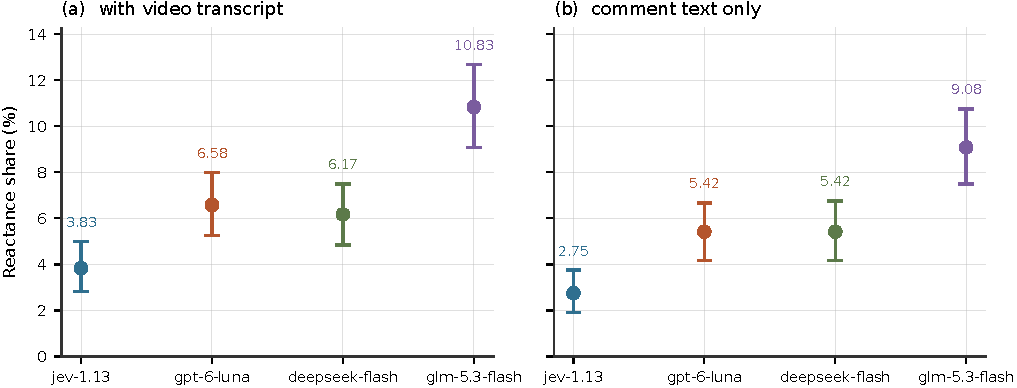
\includegraphics[width=0.9\linewidth]{fig01_prevalence.pdf}
\caption{Prevalence by codebook and condition with 95\%-bootstrap CIs.}
\label{fig:prev}
\end{figure}

\begin{figure}[ht]
\centering
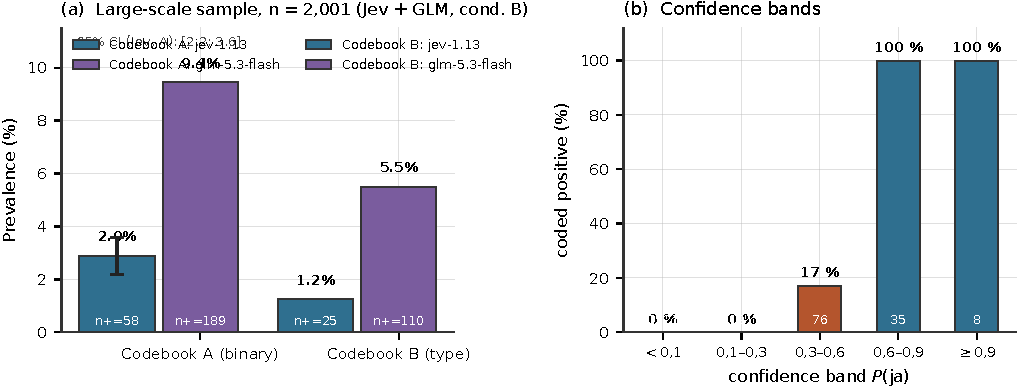
\includegraphics[width=0.9\linewidth]{fig10_bigscale.pdf}
\caption{Large-scale run: prevalence of both codebooks (a) and the
confidence-band structure of the Decisions API (b).}
\label{fig:big}
\end{figure}

\begin{figure}[ht]
\centering
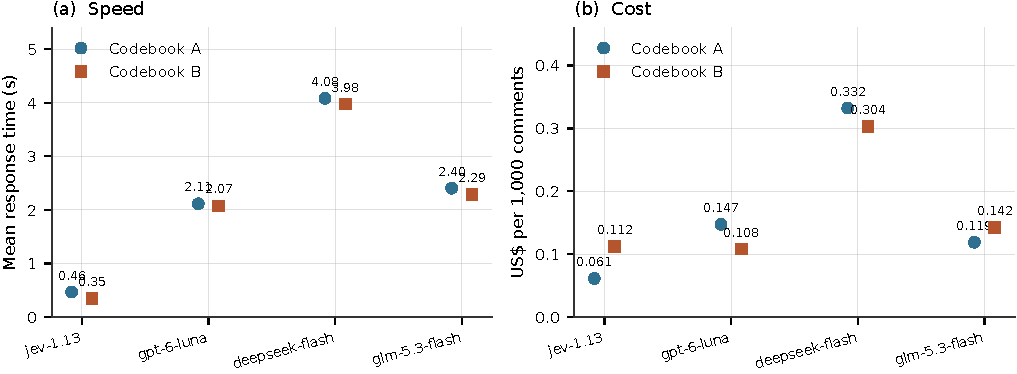
\includegraphics[width=0.85\linewidth]{fig04_cost.pdf}
\caption{Response time (a) and cost (b) per 1{,}000 comments, Condition~A.
Circles: Codebook~A. Squares: Codebook~B.}
\label{fig:cost}
\end{figure}

\subsection{Does the video context help detection?}
\label{sub:transcript}
Dropping the transcript moves the \emph{aggregate} prevalence by less than two
percentage points, in the same direction for all models
($\Delta$ prevalence, Codebook~A, matrix sample: jev 1.1 \,pp,
gpt-6-luna 1.2 \,pp, deepseek 0.8 \,pp, glm 1.8 \,pp;
only Jev's shift reaches the conventional significance level of an exact
McNemar test). The aggregate figure alone does not answer the interesting
question, however, which is whether the \emph{same comments} are classified as
reactant with and without the transcript (Figures~\ref{fig:cmCondA} and
\ref{fig:cmCondB} sit here on purpose). Case-level, the picture is the same in substance: for Jev, 1173 of 1200 comments are classified identically in both conditions (case-level agreement 97.75\%), and only 27 individual comments flip --- 7 gain the reactance label, 20 lose it. The same pattern holds for the other models: flips range from 11 to 59 on Codebook B and from 27 to 121 on Codebook A (Figures~\ref{fig:cmCondA}--\ref{fig:cmCondB}) --- double-digit flip counts in every case, but in absolute terms a small share of the sample. Adding the transcript changes aggregate prevalence only modestly and leaves most item-level classifications unchanged. Without human-labelled ground truth for the transcript-bearing condition, however, we cannot determine whether the remaining label changes improve or reduce validity. For a
cost-sensitive screening pipeline, the limited change in model outputs
provides little evidence that transcript inclusion is necessary.

\begin{figure}[ht]
\centering
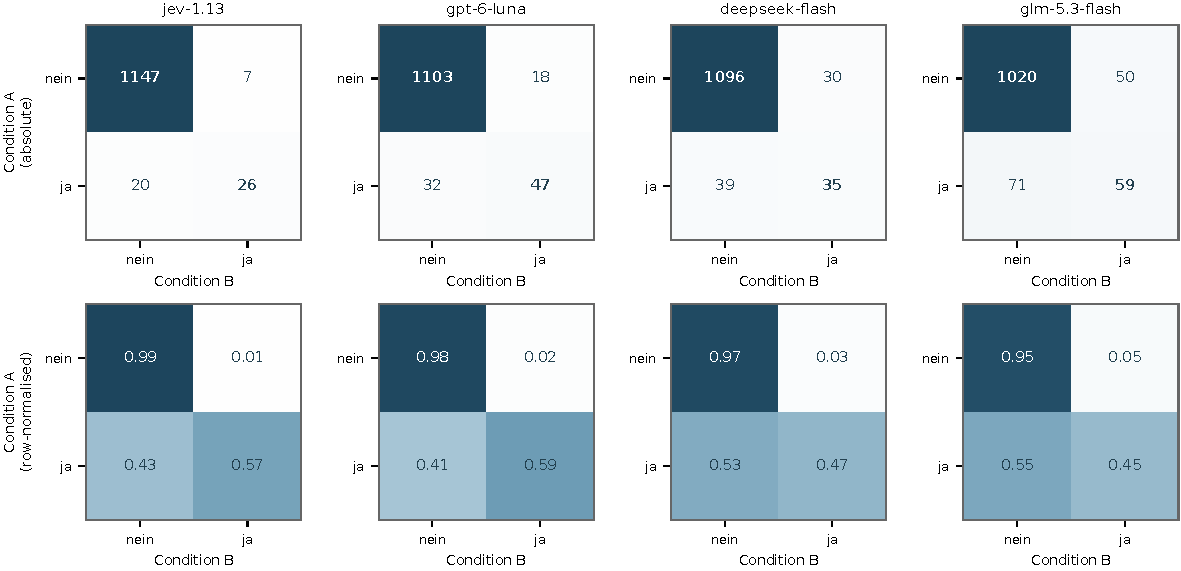
\includegraphics[width=\linewidth]{fig06_confusion_condition_A.pdf}
\caption{Condition~A (with transcript) vs.\ Condition~B (comment only),
Codebook~A: case-level stability of the binary reactance label per model.
Rows = Condition~A, columns = Condition~B.}
\label{fig:cmCondA}
\end{figure}

\begin{figure}[ht]
\centering
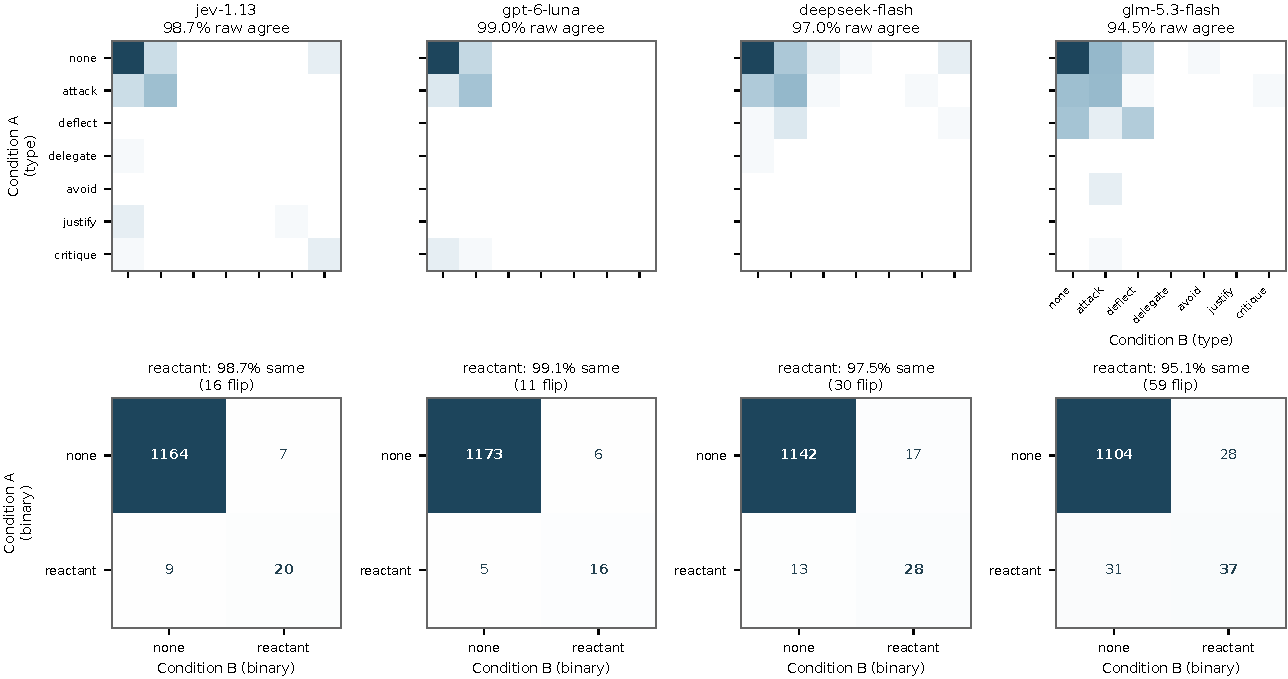
\includegraphics[width=\linewidth]{fig06_confusion_condition_B.pdf}
\caption{Condition~A vs.\ Condition~B, Codebook~B. Top row: the full 7-class
confusion --- does the transcript change the inferred \emph{kind} of
reactance? Bottom row: the binary reactant/none collapse with the four
cells --- are the \emph{same comments} called reactant?}
\label{fig:cmCondB}
\end{figure}

\subsection{GLM-5.3-Flash is the least conservative model}
\label{sec:glm}
The fourth model changes the prevalence picture more than any transcript or
codebook change did. GLM-5.3-Flash marks 10.8\% of the matrix sample as
reactance (Condition~A) --- two to three times the share of the other three
(2.8--6.6\%) --- and flags 189 of the 2001 large-scale comments
where Jev finds 58. This is not better or worse recall in itself; it
is the single largest source of the disagreement structure in
Section~\ref{sec:agree}, and it is a statement about \emph{agreement with the
consensus}, not about which model is correct: GLM deviates most strongly from
its leave-one-model-out consensus of the other three models, which is
exactly what its lower consensus-F1
measures (0.52--0.54, Table~\ref{tab:agree}).

Of the comments only GLM flags, 61 were flagged by no other model in
the matrix sample. The manual audit (Section~\ref{sub:precision}) was drawn
\emph{before} GLM existed and says nothing about this GLM-only stratum; the
v2 audit sample (48 candidates, the GLM-only stratum included) is drawn and
awaiting annotation. No precision claim about GLM-only flags is made here.

\section{Agreement between models}
\label{sec:agree}

With the fourth model in the matrix, the picture sharpens. The three
original models still agree to 94.6--95.1\% raw on Codebook~A, Condition~A,
while GLM-5.3-Flash sits lower: 90.5--91.8\% against each of them, because it
marks roughly twice as many comments as reactance (10.8\% prevalence, the
highest of the four; Section~\ref{sec:freq}). Yet even there the chance-
corrected coefficients tell a two-part story: Cohen's $\kappa$ is low
(0.31--0.59 across all pairs) and Gwet's AC1 high (0.89--0.94). This is not
a contradiction but a base-rate artefact: with 3--11\% positives all models
agree on the easy majority while the few positives split, and $\kappa$
penalises exactly that. \textbf{For these data AC1 --- and, for the binary
task, the per-model F1 of Section~\ref{sub:f1} --- are the appropriate
measures, not $\kappa$ alone.}

All of the following numbers --- raw agreement, the two chance-corrected
coefficients and F1 --- lie on the \emph{same} 0--1 scale. Raw agreement is
the same proportion that the older version plotted as 94.6\% on a separate
percentage axis; expressing it as 0.946 is what lets one axis carry every
quantity and makes the base-rate gap readable at a glance
(Figure~\ref{fig:agree}).

\begin{figure}[ht]
\centering
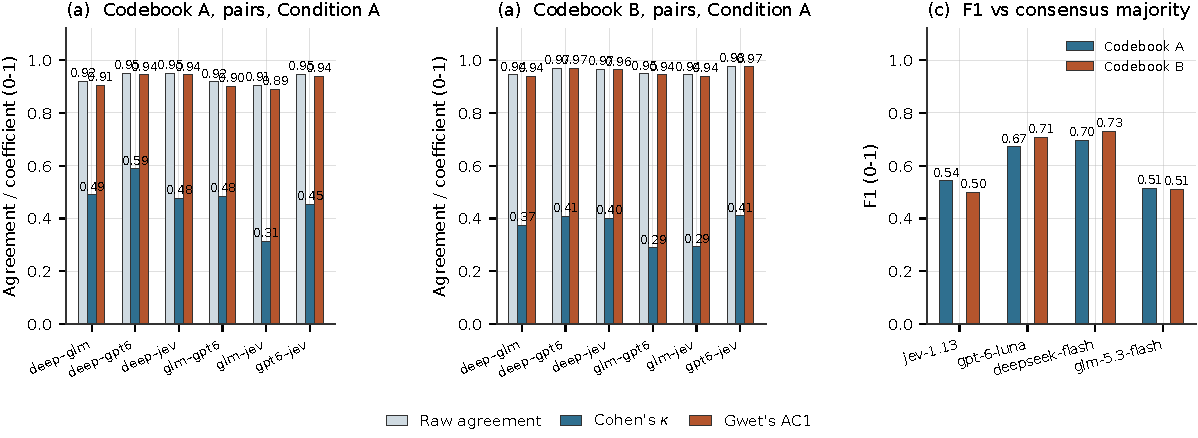
\includegraphics[width=0.98\linewidth]{fig03_agreement.pdf}
\caption{Pairwise agreement on the model pairs (a, b) and per-model F1
against the leave-one-model-out consensus of the other three models (c), all
on a single 0--1 axis: raw
agreement, Cohen's $\kappa$, Gwet's AC1 and F1. The gap between raw
agreement ($\approx$0.91--0.95) and $\kappa$ (0.29--0.59) is the base-rate
artefact; AC1 and, for the binary task, F1 close it.}
\label{fig:agree}
\end{figure}

\begin{table}[htp]
\centering
\caption{Each model against the \emph{leave-one-model-out} consensus of the
other three (Codebook~A, Condition~A). All columns sit on the 0--1 scale ---
raw agreement and F1 next to the two chance-corrected coefficients, plus a
positive-class-specific agreement so the rare-positive overlap is visible
rather than hidden behind the dominant negative class. The reference is a
consensus, not a gold standard: these are agreement numbers, not
correctness numbers.}
\label{tab:agree}
\footnotesize
\setlength{\tabcolsep}{5pt}
\begin{tabular}{lcccccc}
\toprule
Model & $n$ & Raw & F1 & $\kappa$ & AC1 & Pos.\,agree.\\
\midrule
  deepseek-fl. & 1200 & 0.965 & 0.696 & 0.677 & 0.961 & 0.696 \\
  glm-5.3-fl. & 1200 & 0.926 & 0.514 & 0.481 & 0.914 & 0.514 \\
  gpt-6.luna & 1200 & 0.962 & 0.671 & 0.651 & 0.957 & 0.671 \\
  jev-1.13 & 1200 & 0.955 & 0.542 & 0.520 & 0.950 & 0.542 \\
\bottomrule
\end{tabular}
\end{table}

\begin{figure}[htp]
\centering
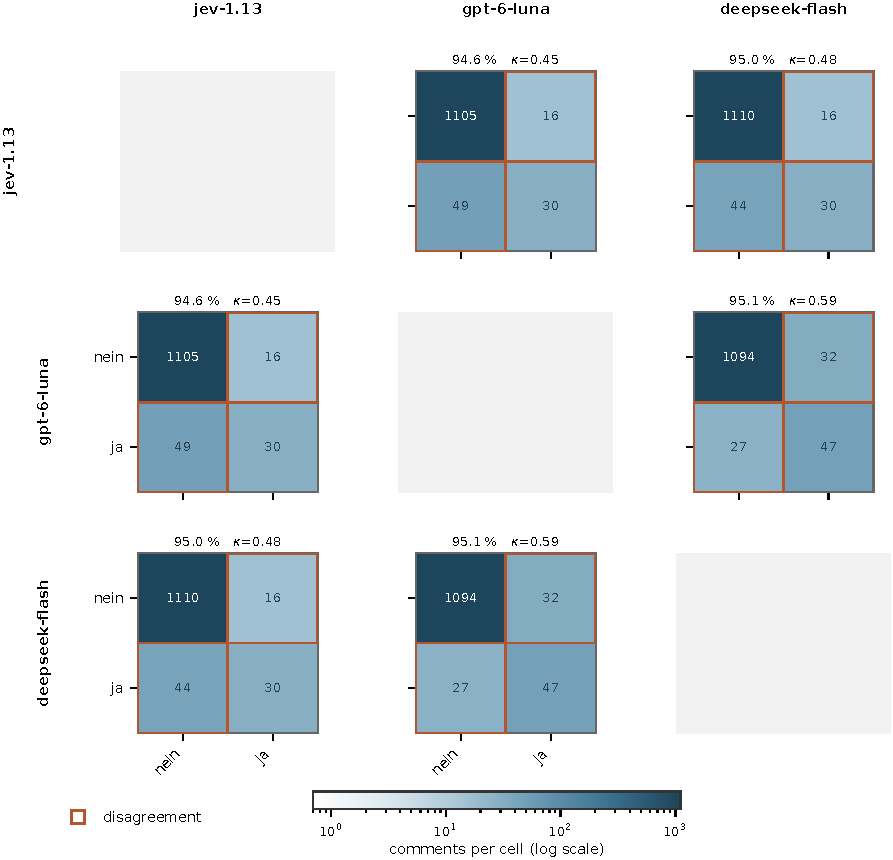
\includegraphics[width=\linewidth]{fig05_confusion_models_A.pdf}
\caption{Confusion matrices model $\times$ model, Codebook~A, Condition~A.
Colour encodes counts; red borders mark disagreement cells.}
\label{fig:cmA}
\end{figure}

\begin{figure}[htp]
\centering
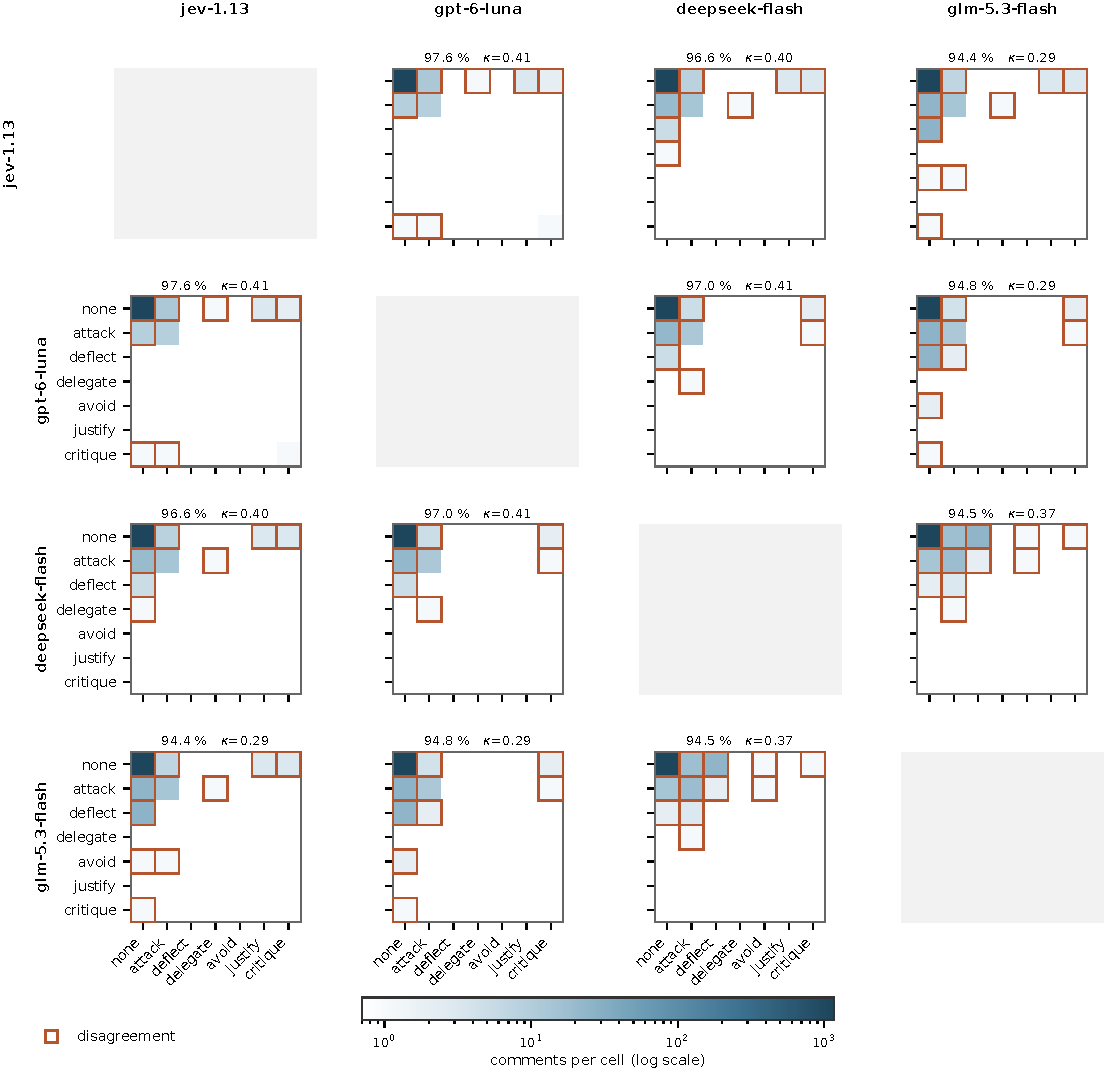
\includegraphics[width=\linewidth]{fig05_confusion_models_B.pdf}
\caption{The same matrix for Codebook~B. Cells carry colour only (no numbers):
the 7-class structure is read visually; values appear in the appended tables.}
\label{fig:cmB}
\end{figure}

\section{Validity: the real bottleneck}
\label{sec:validity}

A prevalence figure is only as solid as the coding rules behind it. Three checks
address this.

\subsection{Precision of positive detection}
\label{sub:precision}
Of the 119 comments marked as reactant by at least one of the \emph{three
original models}, 36 were re-coded manually, stratified by consensus
degree (12 per stratum). \textbf{Scope of this audit: the three original
models.} GLM-5.3-Flash was added to the experiment after the sample was drawn,
so the strata below are ``$k$ of the three original models'' and the audit says
nothing about GLM-only flags. The estimated precision is \textbf{46\%}
(stratum-weighted over the 3-model pool of 119): 92\%
(11/{12} of the cases) at three-model consensus, 50\%
(6/{12}) at a two-model majority and 25\% (3/{12}) for
single-model flags; every value is a point estimate on $n=12$ and the
intervals are Wilson score 95\% intervals (Figure~\ref{fig:audit}). The error is
structured: outrage without a freedom reference; reaction to a claim rather
than to a constraint; named triggers without reactive behaviour.

\begin{figure}[ht]
\centering
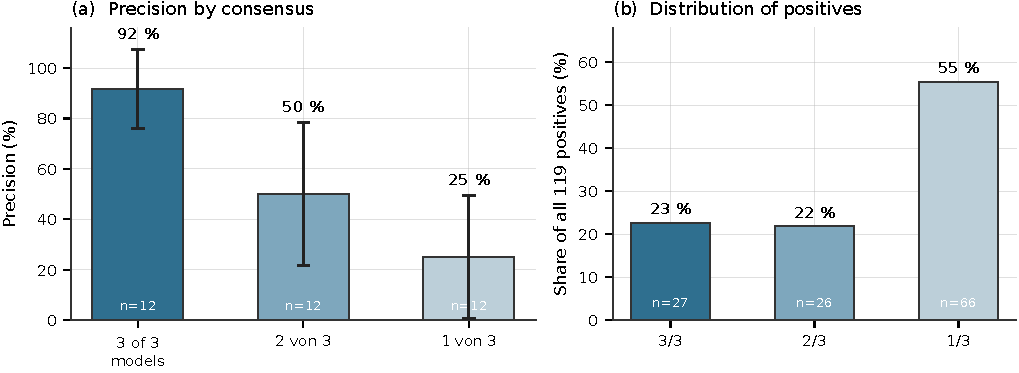
\includegraphics[width=0.9\linewidth]{fig02_audit.pdf}
\caption{Precision by consensus degree (a) and the distribution of the
3-model positives (b); the audit is explicitly the three original models
(GLM was added later and is not covered). Error bars: Wilson score 95\%
intervals on $n=12$ per stratum.}
\label{fig:audit}
\end{figure}

Precision falls sharply with the number of models that agree. Among the cases
flagged by only one of the three original models, 3 of 12 were judged true
positives; among those flagged by all three, 11 of 12 were. Within the audited
cases flagged by a single model, this suggests low precision for isolated
flags, although the estimate rests on a small stratified sample and the
intervals are wide. The positive audit therefore indicates substantial
false-positive contamination, especially in the isolated-flag strata. Raw
model-positive rates should not be read directly as estimates of true
prevalence. Because the audit samples predicted positives rather than the full
comment population, it does not estimate false negatives and cannot establish
whether prevalence is biased upward or downward overall. A v2 audit sample
covering the four-model pool (including the 61 GLM-only flags) is
drawn and awaiting annotation; precision for the four-model strata is a
follow-up, not a number in this report.

\subsection{F1 against the leave-one-model-out consensus}
\label{sub:f1}
F1 is treated as a first-class agreement measure in
Section~\ref{sec:agree}, where it sits next to raw agreement, $\kappa$ and
AC1 (Table~\ref{tab:agree}) rather than in a chapter of its own. The reference
there is a \emph{leave-one-model-out consensus}: each model is compared with
the majority of the other three only, so the evaluated model never votes in
its own reference. It is a consensus, not a gold standard, so F1 reads as how
far a model sits from the consensual position, not how correct it is. At low
prevalence precision and recall pull against each other: Jev has the best
precision but gives up the most recall, and so loses to the chat models
on F1.

\subsection{Codebook A and Codebook B agree --- on both samples}
The error patterns above were translated into a new codebook, together with the
surface-sensitivity finding (Section~\ref{sec:exp}). Gate~2 requires the trigger
to be the \emph{target} of the reaction, not its topic: responding to a claim
is not reacting to a constraint. Gate~3 fixes that politeness markers are
neither trigger nor shield. Both gates sit in the chat instructions \emph{and}
in the Jev criteria, because the Decisions API only returns the criteria.

Two samples, two tables --- deliberately kept apart. On the
\emph{large-scale} sample (2001 comments, Condition~B, Jev and GLM) the two
instruments agree to 98.2\% raw, but the chance-corrected
agreement is only $\kappa=$0.55, with an FP/TP ratio of
0.09 (Jev; Table~\ref{tab:ab}). The very high raw agreement is
driven by both instruments labelling most comments as non-reactant; on the
rare positive class the agreement is moderate once chance is accounted for.
$\kappa$ is computed after collapsing both codebooks to the same binary label
space (A: ja/nein vs.\ B: reactant/none), because comparing the two label
spaces directly would make the expected-agreement term invalid.
The \emph{matrix sample} (1200 comments, all four models) shows the same
pattern per model and condition at n=1200
(Table~\ref{tab:abm}); its aggregate raw agreement is lower simply because the
gate is tested on the harder, transcript-bearing comments.

\begin{table}[htp]
\centering
\caption{Codebook A~$\times$~B agreement, \emph{large-scale sample}
(2001 comments, Condition~B). The n column is part of the point: these
rows are 2{,}001, not the 1{,}200 of the matrix sample.}
\label{tab:ab}
\small
\begin{tabular}{lccccccc}
\toprule
Model & $n$ & both & FP & FN & raw agree & $\kappa$ & FP:TP\\
\midrule
  glm-5.3-fl. & 2001 & 73 & 37 & 116 & 92.3 & 0.45 & 0.51 \\
  jev-1.13 & 2001 & 23 & 2 & 35 & 98.2 & 0.55 & 0.09 \\
\bottomrule
\end{tabular}
\end{table}

\begin{table}[htp]
\centering
\caption{The same agreement, \emph{matrix sample} (1{,}200 comments,
Condition~B, all four models).}
\label{tab:abm}
\small
\begin{tabular}{lccccc}
\toprule
Model & $n$ & both & FP & FN & FP:TP\\
\midrule
  deepseek-fl. & 1200 & 35 & 10 & 30 & 0.29 \\
  glm-5.3-fl. & 1200 & 42 & 23 & 67 & 0.55 \\
  gpt-6.luna & 1200 & 19 & 3 & 46 & 0.16 \\
  jev-1.13 & 1200 & 17 & 10 & 16 & 0.59 \\
\bottomrule
\end{tabular}
\end{table}

\begin{figure}[htp]
\centering
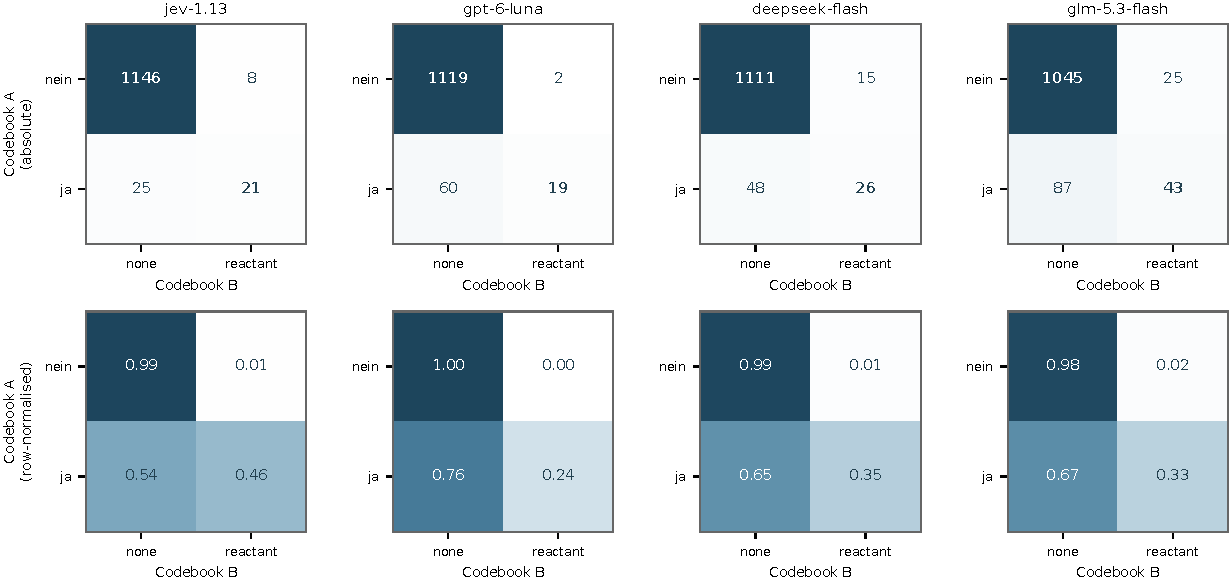
\includegraphics[width=\linewidth]{fig07_confusion_codebook.pdf}
\caption{Confusion of Codebook B (columns) against Codebook A (rows), collapsed
to the binary reactant/none dichotomy, matrix sample.}
\label{fig:cmAB}
\end{figure}

\subsection{Confidence as a corrective}
\label{sub:calib}
Jev returns a class probability $P(\mathrm{ja})$ for every comment; the other
backends do not. Two properties of that number are worth checking separately,
and Figure~\ref{fig:cal} shows both. We are careful about what this
establishes: there is \emph{no independent human-labelled calibration set} in
this experiment, so neither panel is a calibration result in the statistical
sense. The reference in both panels is the leave-one-model-out consensus of
GPT-6-Luna, DeepSeek-V4.1-Flash and GLM-5.3-Flash ---
a proxy, not ground truth --- and the correct reading is
\textbf{probability alignment with the model consensus}, with
probability \emph{discrimination} (do the probability bands separate consensus
positives from non-positives?) being the property that \emph{is} demonstrated.
Brier scores and ECE against human labels require a labelled validation set
and are deliberately not reported here.

\smallskip
\noindent\textbf{(a) Alignment against the consensus majority.} We split
Jev's predictions into ten bins of $P(\mathrm{ja})$ and, in each bin, ask
how often the comment's label agrees with the majority vote of the other
three backends. If Jev's probability were well \emph{aligned} with the
consensus, the observed rate would track the diagonal: predictions of
$P=0.6$ would be majority-reactant about 60\% of the time. The two ends of
the range do track it --- below $P=0.1$ the observed rate is 1\%, above
$P=0.9$ it is 100\% --- but the middle bins sit consistently below the
diagonal, and by a lot in two places: the 0.1--0.2 bin is observed at 4\%
against a mean predicted 14\%, and the 0.3--0.4 bin at 17\% against 35\%.
Roughly a fifth to a third of Jev's mid-range positives are there missed or
refuted by the other three models. Alignment, then, is imperfect in exactly
the region that matters at low prevalence, and the bin sizes printed in
Figure~\ref{fig:cal}(a) show how few comments the upper bins rest on.

\smallskip
\noindent\textbf{(b) The threshold trade-off.} Because $P(\mathrm{ja})$
is meaningful, we can discard low-confidence flags. Raising the threshold
$t$ --- flag only those comments with $P(\mathrm{ja})\geq t$ --- trades
coverage for agreement with the leave-one-model-out consensus: at $t=0.05$
41.2\% of comments are flagged and precision is only 14\%;
at $t=0.6$ precision reaches 79\% but covers only 2.8\% of
the sample. The 70\% line marks the precision of Jev's raw
threshold-free label. Precision, then, is not a property of the model but of
the operating point chosen on this curve --- relative to the consensus of the
other three models, not to a ground truth.

\begin{figure}[ht]
\centering
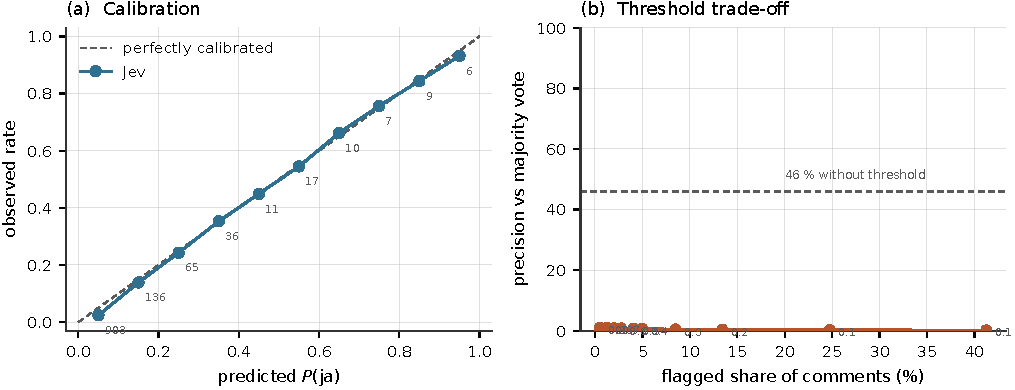
\includegraphics[width=0.94\linewidth]{fig08_calibration.pdf}
\caption{(a) Jev's mean predicted $P(\mathrm{ja})$ within each probability bin
against the observed positive rate of the leave-one-model-out consensus of
GPT-6-Luna, DeepSeek-V4.1-Flash and GLM-5.3-Flash. The grey diagonal indicates
perfect alignment with this consensus proxy; this is not calibration against
human labels. Numbers denote bin sizes. (b) The precision -- coverage trade-off
as the threshold $t$ on $P(\mathrm{ja})$ rises. Precision is measured against
the same leave-one-model-out consensus reference; the horizontal line shows
Jev's threshold-free consensus precision.}
\label{fig:cal}
\end{figure}

\section{Retrospective gated reanalysis: classify type after a Jev-positive gate}
\label{sec:gate}

A production cascade would first run the binary Codebook~A gate and then prompt
only the retained comments with the six reactance types. That second-stage
six-class prompt was \emph{not} run here. Instead, this section is a
\textbf{retrospective gated reanalysis} of predictions that had already been
collected with the original seven-class Codebook~B task on all comments. We
select the comments Jev marked positive under Codebook~A; a stored downstream
\texttt{keine\_reaktanz} answer is treated as rejection of the gate premise,
and the conditional type analysis then considers only the six reactance labels
among retainers. This recombination costs no additional API calls, but it should
not be read as an experimental test of a freshly prompted six-class second
stage. The reanalysis raises two distinct questions: whether downstream
classifiers retain Jev's binary reactance decision, and, conditional on
retaining it, which reactance type they assign.

\medskip
\noindent\textbf{1. Gate retention and rejection.} Jev performs binary reactance
detection over all comments. On the matrix sample, condition~B, the gate lets
through 33 of 1200 comments (2.75\%); on the large-scale
sample 58 of 2001 (2.90\%). Once Jev says ``reactance
present'', a downstream model can still answer
\texttt{keine\_reaktanz}: it \emph{rejects the gate's premise}. How often each
model does this is its own diagnostic (Table~\ref{tab:gatereject},
Figure~\ref{fig:gaterej}): Jev itself re-labels 48\% (16/33) of its own gated comments as \texttt{keine\_reaktanz} in the stored type call; GPT-6-Luna 79\% (26/33), DeepSeek-V4.1-Flash 48\% (16/33), and GLM-5.3-Flash 39\% (13/33). This is a retrospective gate-rejection diagnostic from the existing seven-class predictions; it says nothing about which \emph{type} the retainers then choose.

\begin{table}[htp]
\centering
\caption{Gate retention vs.\ rejection in the retrospective reanalysis: of the
33 comments Jev's gate selected (matrix sample, Condition~B), how many
does each model's already-collected Codebook~B prediction retain as reactant
(assign one of the six types) and how many does it label
\texttt{keine\_reaktanz}?}
\label{tab:gatereject}
\small
\begin{tabular}{lcccc}
\toprule
Model & $n$ gated & retain & reject & reject\%\\
\midrule
  jev-1.13 & 33 & 17 & 16 & 48\% \\
  gpt-6.luna & 33 & 7 & 26 & 79\% \\
  deepseek-fl. & 33 & 17 & 16 & 48\% \\
  glm-5.3-fl. & 33 & 20 & 13 & 39\% \\
\bottomrule
\end{tabular}
\end{table}

\begin{figure}[ht]
\centering
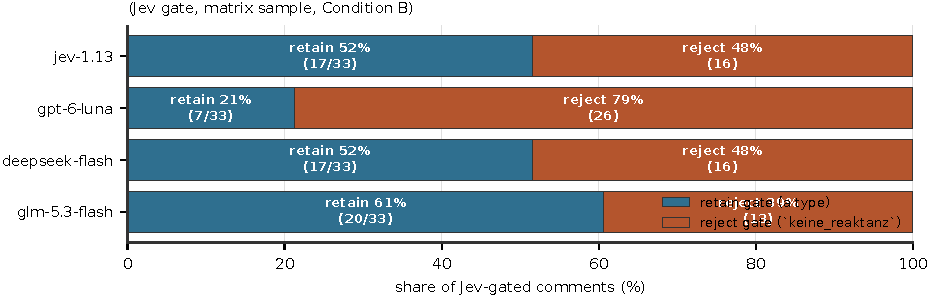
\includegraphics[width=0.9\linewidth]{fig13_gate_rejection.pdf}
\caption{Retrospective gate retention vs.\ rejection per model (matrix sample,
Condition~B).}
\label{fig:gaterej}
\end{figure}

\medskip
\noindent\textbf{2. Conditional six-class type agreement.} For the analysis
conditional on retaining the gate, \texttt{keine\_reaktanz} is excluded and
the remaining label space contains the six reactance types. Given that two
models both retain the gate, which types do they confuse?
Figure~\ref{fig:gatecm} is that six-class grid; each cell carries its
conditional $n$, because support differs from pair to pair once rejections are
removed. The retained type calls are dominated by
\texttt{konfrontation\_angriff} (attack), with the other five types at single
digits in total (support annotated in Figure~\ref{fig:gatecm}), and the pairwise
conditional support is tiny ($n$ between 5 and 14).
Type-level agreement therefore is \emph{descriptive only}: raw pairwise
agreement ranges from 85 to 100\% ($\kappa$ 0.00--1.00; on the
same gated set the unconditional seven-class predictions agree 58--70\%,
$\kappa$ 0.18--0.46). A global six-class $\kappa$ on near-empty classes is
not a robust summary.

\begin{figure}[ht]
\centering
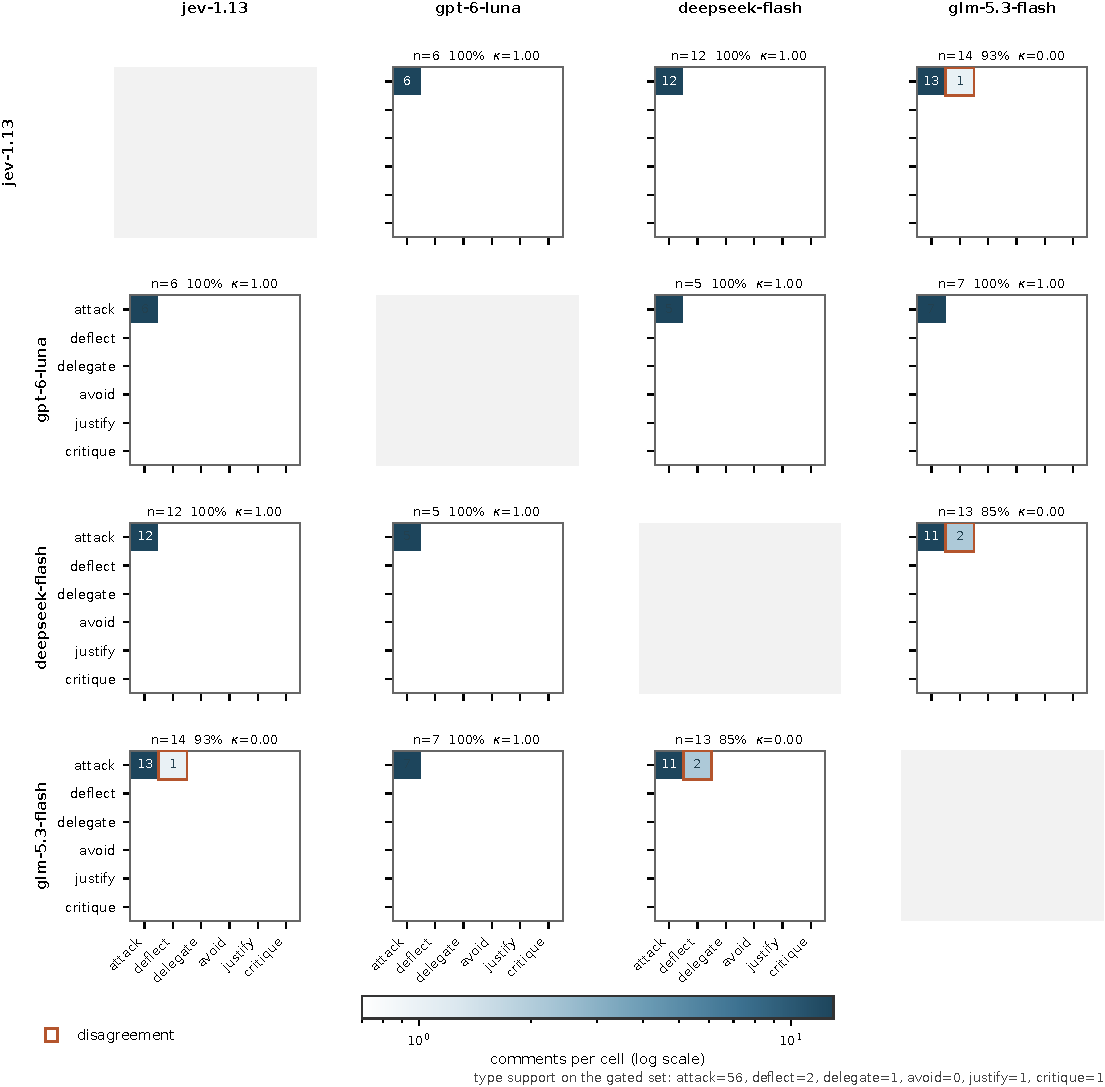
\includegraphics[width=\linewidth]{fig11_gate_confusion.pdf}
\caption{Conditional six-class type confusion in the retrospective gated
reanalysis (matrix sample, Condition~B): rows and columns are the four models'
stored type labels, restricted to comments on which both models retained Jev's
positive gate. Each cell carries its conditional $n$; per-type support is
annotated below.}
\label{fig:gatecm}
\end{figure}

\medskip
\noindent\textbf{3. Consensus among the retaining models.} The plurality is
recomputed on the six types among the models that \emph{retained} the gate.
Gate acceptance and conditional type consensus are distinct quantities
(Figure~\ref{fig:gatemaj}): 5 of 33 comments have all four models
retaining the gate and 7 are rejected by all, while \emph{among the
retainers} the type label is a plurality of four (5), three (6), two
(6) or one (8), with 1 explicit ties. Requiring three-or-more
models to retain the gate keeps 36\% of the gated stream. On the
large-scale sample the gate is more selective (58 of 2001
comments), of which 18 reach a plurality of the retaining models on the
type.

\begin{figure}[ht]
\centering
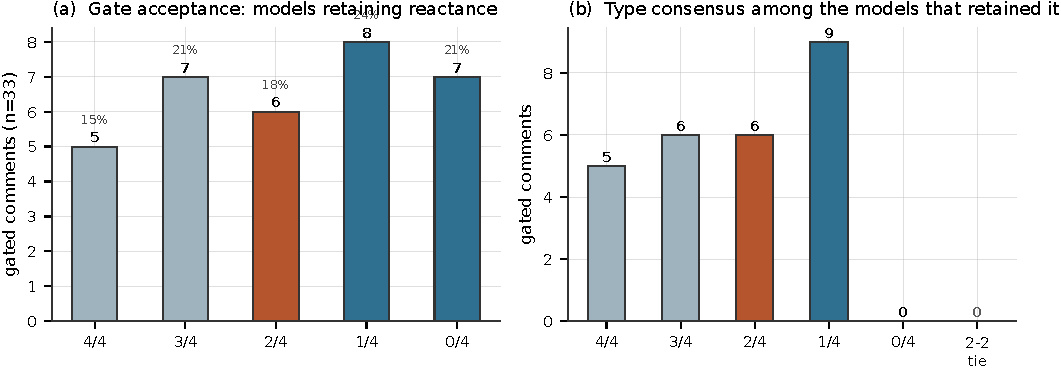
\includegraphics[width=0.9\linewidth]{fig12_gate_majority.pdf}
\caption{Retrospective gated reanalysis, matrix sample, Condition~B.
(a)~Gate acceptance: how many of the four stored Codebook~B predictions retain
each Jev-gated comment as reactant. (b)~Conditional type consensus among the
models that retained it, with ties shown separately.}
\label{fig:gatemaj}
\end{figure}

The substantive descriptive result is that disagreement on Jev-gated cases is
not only type disagreement: a substantial share concerns whether the stored
Codebook~B prediction accepts the reactance premise at all. A production
six-class second-stage prompt remains to be tested directly.

\section{Two validation experiments}
\label{sec:exp}

\subsection{Repeat stability and position robustness}
Identical inputs were coded twice on oversampled positives and a matched negative control. Jev is 98.47\% stable overall, with 100.0\% on the control and 96.94\% on the positives; flips sit at the decision boundary p(ja)$\approx$0.31. Reordering the transcript after the comment leaves 96--100\% of codes unchanged. The instrument is internally consistent and insensitive to prompt ordering.

\subsection{Surface/framing sensitivity}
\label{sub:surf}
The experiment applies three deterministic perturbations to the comment text.
T1 removes emphasis. T2 first applies T1 and then adds a fixed opener/closer;
T3 first applies T1 and then removes selected filler particles. These
transformations preserve the lexical core but are not guaranteed to be
semantically or pragmatically neutral, especially T2, whose framing changes
tone and can contain an imperative. Table~\ref{tab:surf} should therefore be
read as a \emph{sensitivity diagnostic}, not as a pure meaning-preserving
invariance test. De-emphasis is highly stable; filler removal is somewhat less
stable; the T2 framing intervention is most disruptive, leaving only 62--78\%
of labels unchanged in the three original-model positive-pool strata. This
finding motivated Gate~3, but does not by itself establish that politeness
alone caused the flips.

\begin{table}[htp]
\centering
\caption{Surface/framing sensitivity (Jev, Codebook A, Condition A): share of
labels unchanged relative to the original. Historical strata are defined by
the original three-model pool. T2 and T3 are compositional interventions that
include T1 de-emphasis.}
\label{tab:surf}
\setlength{\tabcolsep}{5pt}
\resizebox{\linewidth}{!}{%
\begin{tabular}{lccccc}
\toprule
Stratum & $n$ & emphasis & T1+framing & T1+filler removal & all three\\
\midrule
  3 von 3 & 27 & 96\% & 78\% & 93\% & 78\% \\
  2 von 3 & 26 & 92\% & 62\% & 88\% & 62\% \\
  1 von 3 & 35 & 97\% & 77\% & 89\% & 69\% \\
  Kontrolle & 105 & 100\% & 98\% & 100\% & 98\% \\
\bottomrule
\end{tabular}}
\end{table}

\begin{figure}[ht]
\centering
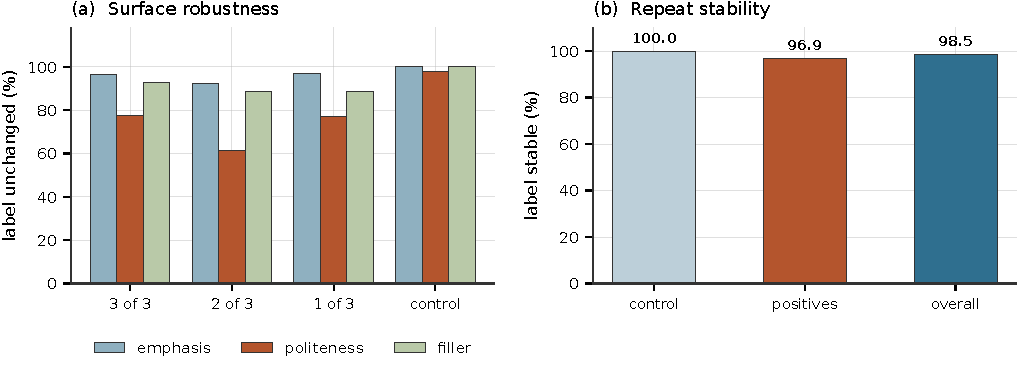
\includegraphics[width=0.94\linewidth]{fig09_reliability.pdf}
\caption{Surface/framing sensitivity (a) and repeat stability (b), Jev,
Codebook A, Condition A.}
\label{fig:rel}
\end{figure}

\section{Discussion}
\noindent\textbf{Prevalence, not effect.} The classifiers flag reactance
rarely in the studied corpus. That is a finding, not a flaw --- and it shifts
the work from measuring
frequency to validating it. At low prevalence the question is not which model
more often says yes, but whether a label carries at all.

\medskip
\noindent\textbf{The context work is low-priority.} Adding the transcript
changes aggregate prevalence only modestly and leaves most item-level
classifications unchanged (Section~\ref{sub:transcript}): most classifications remain unchanged, but item-level flips range from 11 to 59 per model on Codebook B and from 27 to 121 on Codebook A. For a cost-sensitive screening pipeline the limited change in model outputs provides little evidence that transcript inclusion is necessary; the experiment measures output stability, not demonstrated accuracy.
The most practical message for a pipeline over 6.7~million comments is that
the comment text appears sufficient for screening, while the transcripts
remain available for the intervention side of the project.

\medskip
\noindent\textbf{Cascades instead of monoliths.} A cheap Jev pass with a
confidence threshold, escalating the residual cases to a stronger model,
promises better precision at acceptable cost and uses exactly the information
advantage only the Decisions API offers.

\medskip
\noindent\textbf{A ground truth is still missing.} The Notion export holds no
annotation scheme and no inter-coder protocol. The re-coding in
Section~\ref{sub:precision} and the F1 figures in Section~\ref{sub:f1} are a
first step, but were produced by the assistant and replace no supervised double
coding with a training phase. The $\kappa$- and AC1-values measure consistency
among models, not correctness against human coding. In
Section~\ref{sub:precision}, ``precision'' is the stratum-weighted estimate
from the three-model audit; in Figure~\ref{fig:cal} and the threshold analysis,
``precision'' is agreement with the leave-one-model-out model consensus. F1
against the majority is likewise an agreement measure. Until a labelled
validation set exists, none of these quantities is a substitute for human-ground-truth
accuracy.

\section{Limitations}
The sample was built for the method question, not as a representative sample:
comments under 25 characters, replies and non-public comments are excluded, and
party cells are too small for group comparisons. The transcripts come from
automatic speech recognition with substantial errors; Condition~A suffers more
than Condition~B. The precision estimate rests on 36 cases and one coder (the
assistant), on the original three-model pool only; the 4-model audit (including
the GLM-only flags) is sampled and pending. The majority vote is not a ground
truth. The gated six-class results are a retrospective conditional reanalysis
of already-collected seven-class predictions, not a fresh six-class second
stage; they run on 33 conditional observations in the matrix sample, most of
them one type, so the type-level results are descriptive. The surface/framing
perturbations are deterministic but not guaranteed pragmatically neutral, so
their results identify sensitivity rather than a causal effect of politeness.
Finally, the confidence bands of the Decisions API are sharply bimodal ---
1{,}521 comments below $p=0.1$ are never positive, 43 above $p=0.6$ always are
--- so the threshold aligned here is not yet transferable to new data.

\appendix
\section{Detailed tables}
\label{app:tables}
The full model-pair, condition-A/B and codebook matrices are too large for the
main body; they and the per-request logs are regenerable from the repository
(Section~\ref{sec:repro}).

\section{Codebook}
\label{app:codebook}
\textbf{Codebook A -- binary.} \texttt{ja} iff both (1) a perceived restriction
of one's own freedom (trigger dimensions A--D) and (2) an affective or
behavioural counter-reaction. Otherwise \texttt{nein}.

\medskip
\noindent\textbf{Codebook B -- seven types.} The eight archetypes of the
DemocraGPT typology, condensed to disjoint labels:
\begin{itemize}\itemsep2pt
\item \texttt{konfrontation\_angriff} -- destructiver und konstruktiver Angreifer
\item \texttt{ablenkung\_whataboutism} -- aggressiver Ablenker und Ablenkungs-Stratege
\item \texttt{delegierung\_hilflosigkeit} -- hilfloser Delegierer
\item \texttt{vermeidung\_rueckzug} -- vermeidender Rechtfertiger
\item \texttt{reflektierte\_rechtfertigung} -- reflektierter Rechtfertiger
\item \texttt{konstruktive\_kritik} -- konstruktiver Kritiker
\item \texttt{keine\_reaktanz} -- no reactance
\end{itemize}

\medskip
\noindent\textbf{Gates.} Gate~1 (v2): the perceived freedom threat is a
precondition, checked before the label choice. Gate~2 (v3): the trigger must be
the target of the reaction. Gate~3 (v3): politeness markers are neither trigger
nor shield. All gates stand in the chat instructions \emph{and} in the Jev
criteria.

\section{Reproduction}
\label{sec:repro}
\begingroup\footnotesize
\begin{verbatim}
git clone https://github.com/DanielMatterTUM/democragpt-experiments
cd democragpt-experiments
pip install -r requirements.txt -r requirements-analysis.txt
export OPENROUTER_API_KEY=...
python3 src/build_dataset.py --target 1200 --n-accounts-per-party 8 \
    --out sample_matrix
python3 src/run_benchmark.py --models jev-1.13 gpt-6-luna \
    deepseek-v4.1-flash glm-5.3-flash --codebooks A B \
    --conditions A B --workers 12 --run-name full
python3 src/dedup_one.py requests_full
# glm on the large-scale sample (condition B only)
python3 src/run_benchmark.py --models glm-5.3-flash --codebooks A B \
    --conditions B --sample sample_big.jsonl --run-name glm_big
# analysis (all four steps before the figures, the report asserts their meta)
python3 src/analyze_extended.py
python3 src/analyze_big.py
python3 src/analyze_gate.py
python3 src/score_audit.py
python3 src/make_audit_sample_v2.py   # draws the pending 4-model audit sample
python3 src/exp_reliability.py 45
python3 src/exp_paraphrase.py 35
python3 src/make_report.py
python3 src/figures.py
python3 src/validate_report.py        # consistency check, fails the build
python3 src/generate_latex.py
cd report && ./make.sh
\end{verbatim}
\endgroup

\printbibliography[heading=secbib]
\end{document}
